\documentclass[a4paper,12pt]{article}

% Paquetes básicos
\usepackage[utf8]{inputenc}
\usepackage[T1]{fontenc}
\usepackage[spanish]{babel}
\usepackage{graphicx}
\usepackage{xcolor}
\usepackage{lipsum}
\usepackage{geometry}
\geometry{top=3cm, bottom=3cm, left=2.5cm, right=2.5cm}

% Paquetes para diseño
\usepackage{titlesec}
\usepackage{fancyhdr}
\usepackage{amsmath}
\usepackage{amssymb}
\usepackage{hyperref}
\usepackage{tcolorbox}
\usepackage{float}

% Paquetes para el entorno lstlisting
\usepackage{listings}
\usepackage{inconsolata}

\usepackage{tocbibind} % Para incluir subsubsubsections en el índice
\usepackage{titlesec}  % Para ajustar la numeración de las secciones
\setcounter{tocdepth}{5} % Ajusta la profundidad del índice
\setcounter{secnumdepth}{5} % Ajusta la profundidad de la numeración

% Configuración de la numeración para \paragraph
\titleformat{\paragraph}
{\normalfont\normalsize\bfseries}{\theparagraph}{1em}{}
\titlespacing*{\paragraph}{0pt}{3.25ex plus 1ex minus .2ex}{1.5ex plus .2ex}

% Paquete para fondo
\usepackage{background}

% Configuración de lstlisting
\lstset{
    language=Python,
    basicstyle=\ttfamily\small,
    keywordstyle=\color{blue}\bfseries,
    stringstyle=\color{teal},
    commentstyle=\color{gray}\itshape,
    numbers=left,
    numberstyle=\tiny\color{gray},
    backgroundcolor=\color{black!5},
    frame=single,
    rulecolor=\color{black!50},
    breaklines=true,
    captionpos=b,
    showstringspaces=false
}

% Configuración de título
\titleformat{\section}{\normalfont\Large\bfseries}{\thesection}{1em}{}

% Información del documento
\title{
    \vspace{-2cm}
    
\includegraphics[width=0.3\textwidth]{images/fccee.jpg} \\ % Cambia el logo si es necesario
    \LARGE Ingeniería Informática + ADE\\
    \large Universidad de Granada (UGR)\\[1cm]
}
\author{\textbf{Autor:} Ismael Sallami Moreno}
\date{\textbf{Asignatura:} Resúmenes de Contabilidad Financiera I Tema 5: Inmovilizaciones materiales
}
\usepackage{mathpazo}
\pagestyle{fancy}
\fancyhf{}
\fancyhead[L]{\textbf{\textsf{\leftmark}}}
\fancyhead[R]{\textbf{\textsf{\thepage}}}
\fancyfoot[C]{\thepage}
\usepackage{enumitem}

% Configuración del fondo
\backgroundsetup{
    scale=1,
    color=black,
    opacity=0.2,
    angle=0,
    position=current page.south,
    vshift=0pt,
    hshift=0pt,
    contents={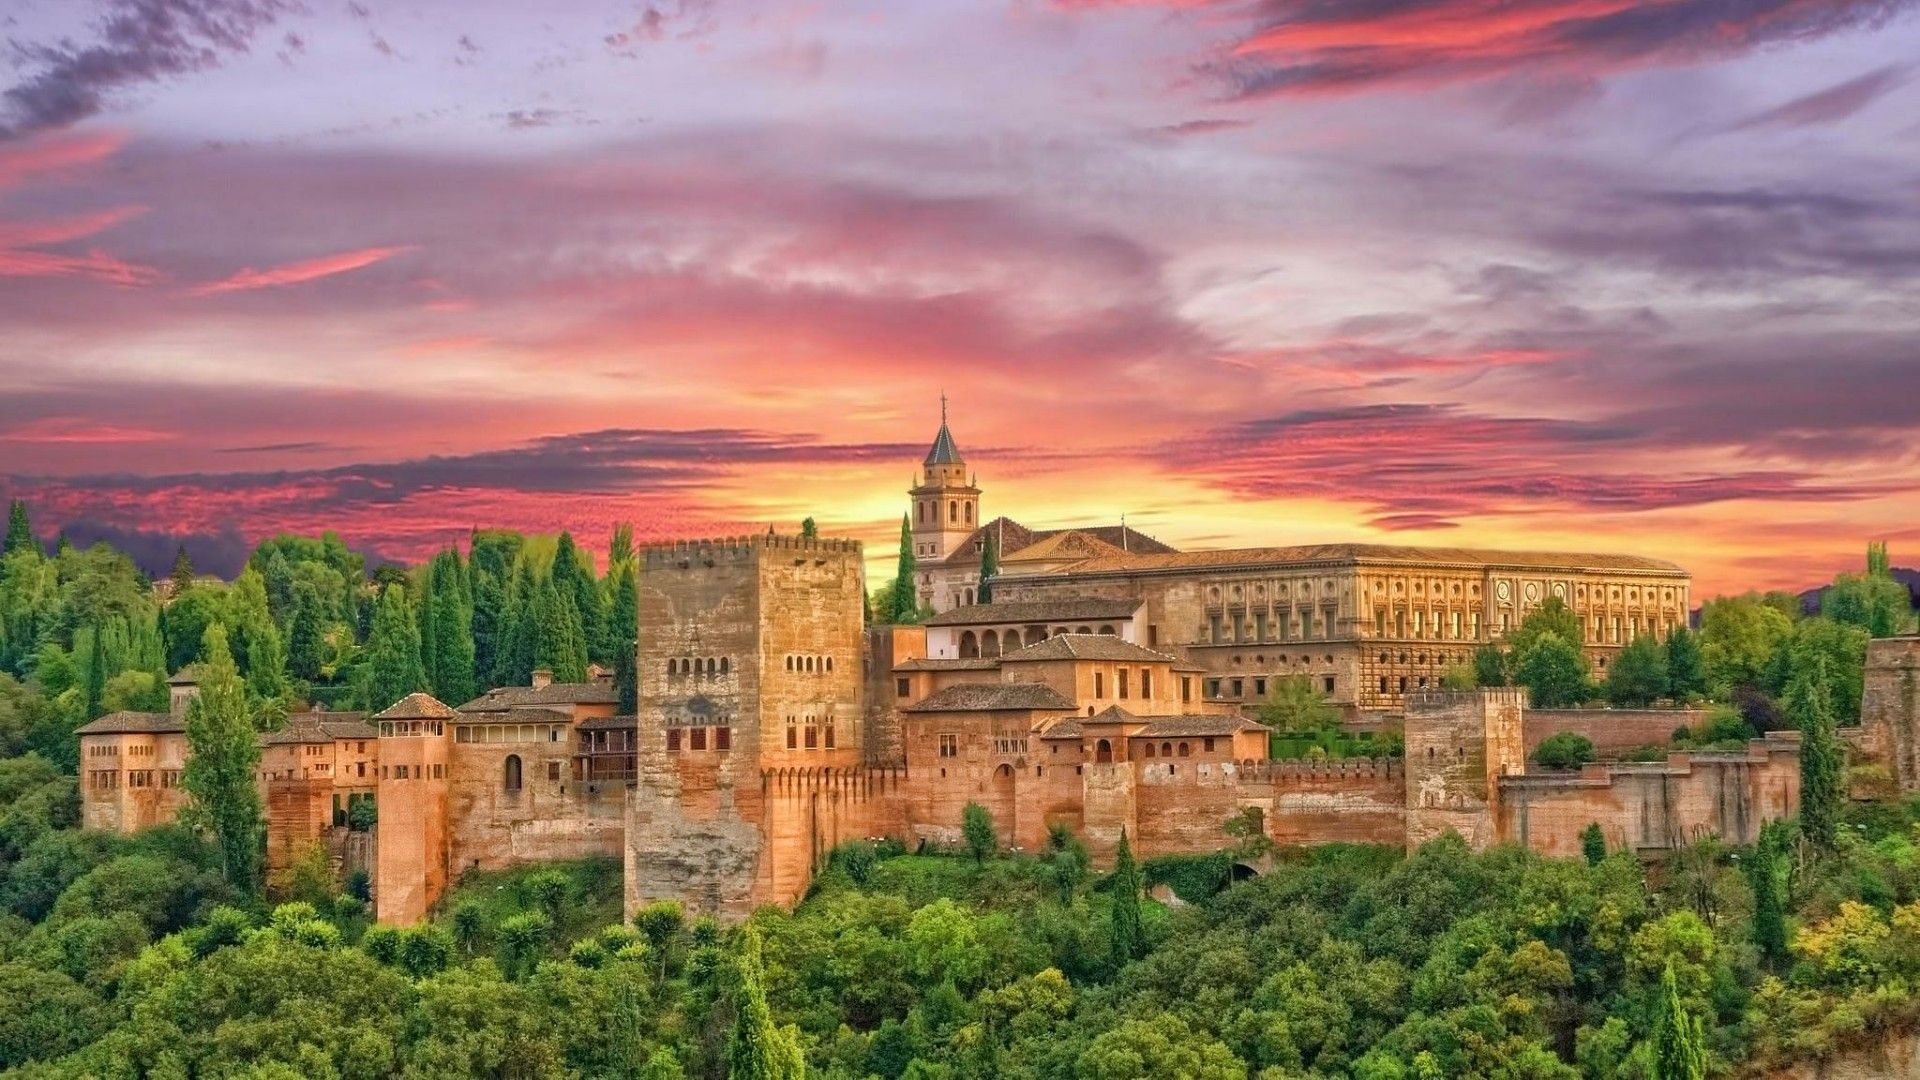
\includegraphics[width=\paperwidth,height=\paperheight,keepaspectratio]{images/granada.jpg}}
}

% Inicio del documento
\begin{document}

% Portada
\maketitle
\thispagestyle{empty}

\begin{center}
    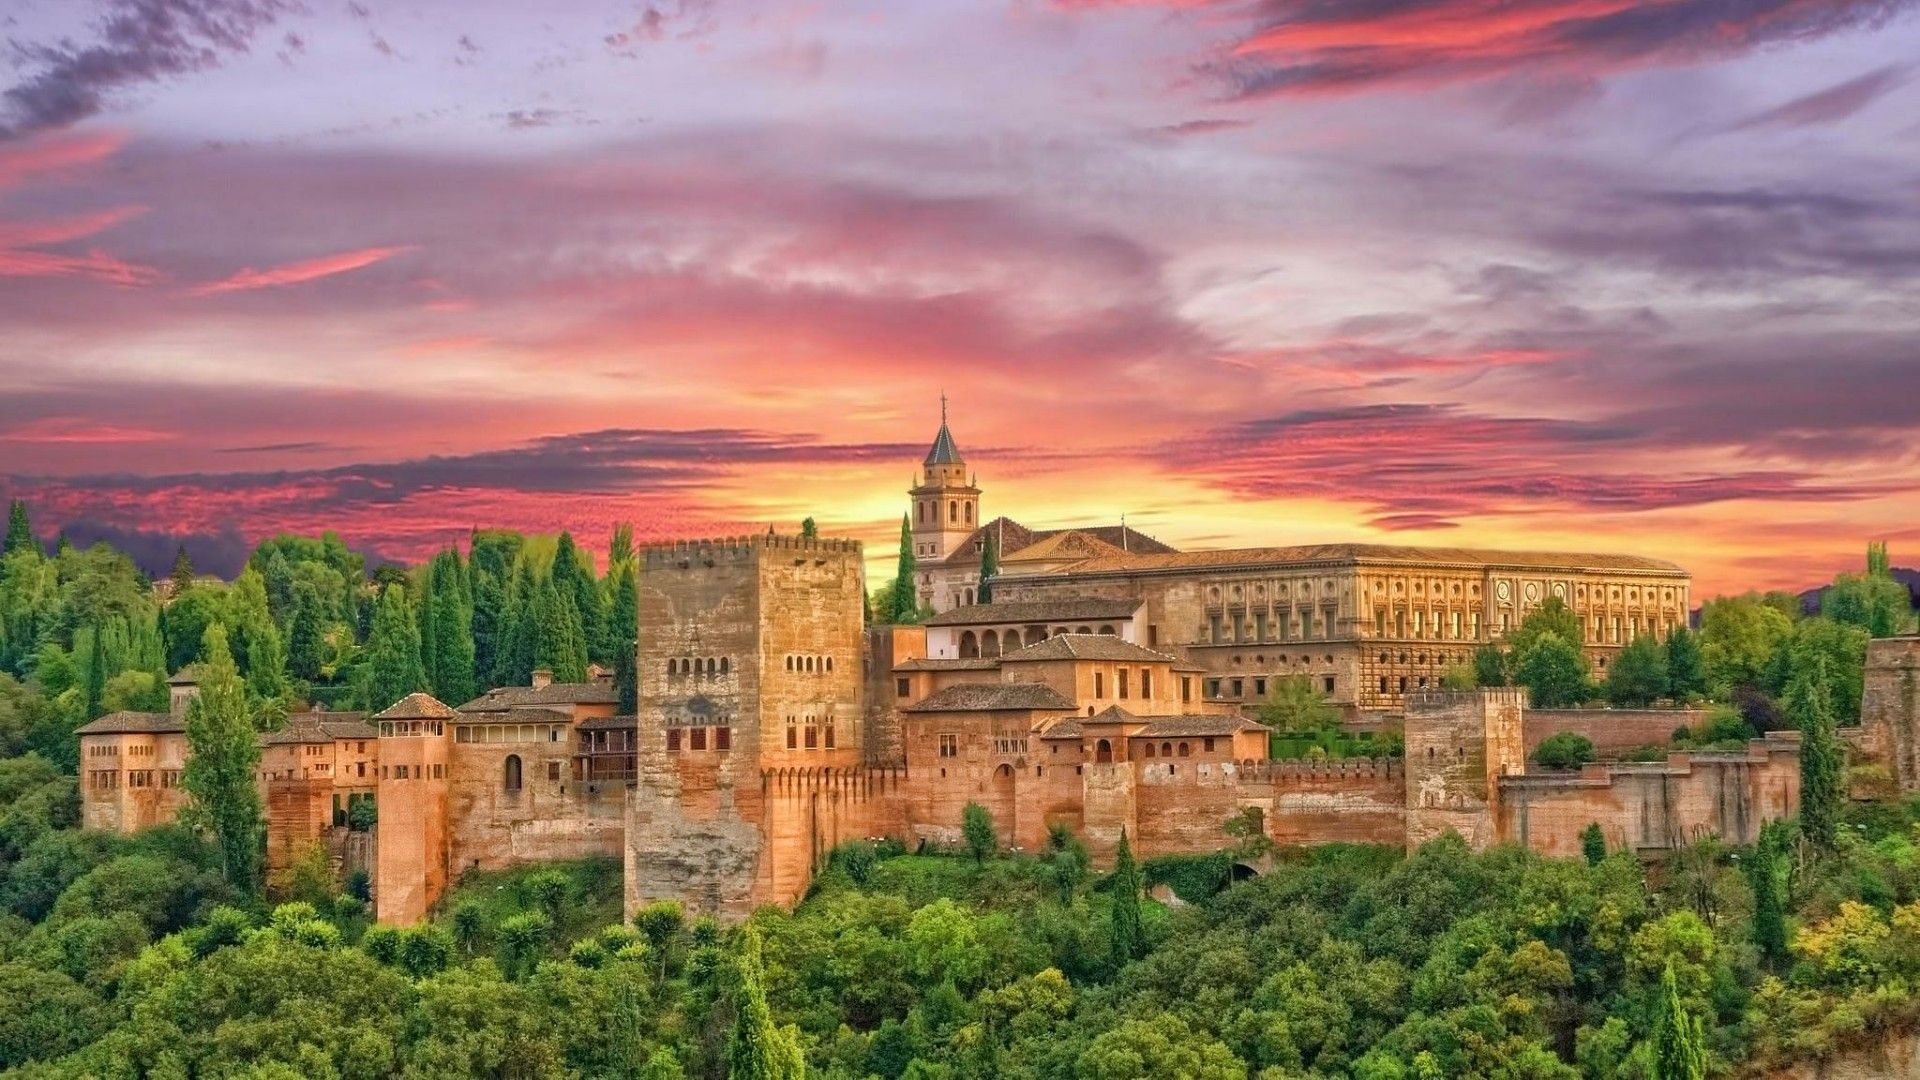
\includegraphics[width=\textwidth,height=0.4\textheight,keepaspectratio]{images/granada.jpg} \\ % Añade tu imagen de fondo
    \vfill
\end{center}

\newpage

% Índice (opcional)
\tableofcontents
\newpage

\section{Concepto, características y clasificación del inmovilizado}

\subsection{Concepto de inmovilizado}
Bienes, derechos y otros recursos controlados económicamente por la empresa, resultantes de sucesos pasados, de los que se espera que la empresa obtenga beneficios o rendimientos económicos en el futuro.

\subsection{Definición de activo no corriente}
Comprende los activos destinados a servir de forma duradera en las actividades de la empresa, incluidas las inversiones financieras cuyo plazo de vencimiento sea superior a un año.

\subsubsection{Características del activo no corriente}
\begin{itemize}
    \item largo plazo
    \item no están destinados a ser vendidos
    \item incluye las inversiones financieras a largo plazo
    \item se deprecia de manera irreversible y sistemática (amortización técnica) y también se puede depreciar de modo reversible (deterioros de valor)
\end{itemize}

\subsection{Definición de activo corriente}
Comprende los activos vinculados al ciclo normal de explotación que la empresa espera a vender, consumir o realizar. El ciclo de explotación no excederá un año.

\subsection{Ciclo normal de explotación}
Periodo que transcurre entre dos momentos de tiempo: 
\begin{enumerate}
    \item momento de adquisición de bienes que se invierten (proceso productivo)
    \item realización de los bienes de manera efectiva(recuperación de la inversión)
\end{enumerate}

\subsection{Clases de inmovilizado}

En función del subgrupo:
\begin{itemize}
    \item 20: Inmovilizado intangibles
    \item 21: Inmovilizado materiales
    \item 22: Inmovilizado inmobiliarias
    \item 23: Inversiones materiales en curso
    \item 24: Inversiones financieras en partes vinculadas
    \item 25: Inversiones financieras a largo plazo
    \item 26: Fianzas y depósitos constituidos a largo plazo
    \item 27: Amortización acumulada del inmovilizado
    \item 28: Deterioro de valor del Inmovilizado
\end{itemize}

\section{Concepto y características del inmovilizado material}
Elementos de activos tangibles como muebles, inmuebles y bienes, las características principales son:

\begin{itemize}
    \item uso a largo plazo en la producción de bienes y servicios de la empresa
    \item no se quieren vender, pero pueden enajenar operaciones extraordinarias
    \item pérdidas de valor por uso, paso del tiempo, obsolencia tecnológica, pérdidas de valor reversibles
\end{itemize}

\textbf{Grupo 21 Inmovilizados materiales:
}\begin{itemize}
    \item 210 Terrenos y bienes naturales
    \item 211 Construcciones
    \item 212 Instalaciones técnicas
    \item 213 Maquinaria
    \item 214 Utillaje
    \item 215 Otras Instalaciones
    \item 216 Mobiliario
    \item 217 Equipos para procesos de Información
    \item 218 Elementos de transporte
    \item 219 Otro inmovilizado material
\end{itemize}

\textbf{Grupo 23 Inmovilizaciones materiales en curso:
}\begin{itemize}
    \item 230 adaptaciones de terrenos y bienes naturales
    \item 231 Construcciones en curso
    \item 232 Instalaciones técnicas en montaje
    \item 233 Maquinaria en montaje
    \item 237 Equipos para procesos de información en montaje
    \item 239 anticipos para inmovilizaciones materiales
\end{itemize}

Distincción entre estos dos grupos es la puesta en \textbf{condiciones de funcionamiento.}

\section{Criterios Generales de Reconocimiento y Valoración}
\subsection{Cuestiones previas}
\begin{itemize}
    \item \textbf{¿Qué es el reconocimiento de un activo?} reflejo en las cuentas anuales según los criterios establecidos para ello.
    \item \textbf{¿Qué criterios deben cumplirse para reconocer un activo según el Marco Conceptual del PGC?} rendimientos futuros  y valoriación fiable.
    \item \textbf{Valoración inicial y valoriación posterior.} Cuando se incorpora por primera vez y el resto de la vida útil.
\end{itemize}

\subsection{Criterios de valoriación según la forma de adquisición del inmovilizado}
\begin{table}[H]
\centering
\caption{Criterios de valoración según la forma de adquisición del inmovilizado}
\begin{tabular}{|p{4cm}|p{4cm}|p{8cm}|}
\hline
\textbf{ORIGEN} & \textbf{CRITERIO DE VALORACIÓN} & \textbf{CÁLCULO/COMPONENTES} \\
\hline
A) Adquisición onerosa (pago de precio al exterior) & Precio de adquisición & 
\begin{itemize}
    \item Importe o Precio recogido en la factura del proveedor
    \item + Valor razonable otras contraprestaciones
    \item + Gastos adicionales directos hasta fecha de puesta en condiciones de funcionamiento del activo
    \item + Gastos financieros por financiación ajena, hasta la fecha de puesta en condiciones de funcionamiento y siempre que la misma dure más de un año
    \item - Todos los descuentos o rebajas concedidas por el proveedor
    \item + Estimación inicial del Valor actual de los gastos futuros por desmantelamiento o retiro
    \item + IVA no deducible (no recuperable)
\end{itemize} \\
\hline
B) Producción por la propia empresa & Coste de producción & 
\begin{itemize}
    \item Valor de materias primas y materiales empleados
    \item + Costes directos imputables
    \item + Proporción razonable de los costes indirectos
    \item + Gastos financieros directos por financiación ajena, hasta la fecha de puesta en condiciones de funcionamiento y siempre que la fabricación dure más de un año
    \item + Estimación inicial del Valor actual de los gastos futuros por desmantelamiento o retiro
\end{itemize} \\
\hline
\end{tabular}
\end{table}

\begin{table}[H]
\centering
\begin{tabular}{|p{4cm}|p{4cm}|p{6cm}|}
\hline
\textbf{ORIGEN} & \textbf{CRITERIO DE VALORACIÓN} & \textbf{CÁLCULO/COMPONENTES} \\
\hline
C) Donación o legado & Valor razonable & 
\begin{itemize}
    \item Valor de mercado, o estimación fiable si no existe mercado organizado, activo y líquido
\end{itemize} \\
\hline
D) Permutas y aportaciones de capital no dinerarias & Valor razonable, o bien Valor contable & 
\begin{itemize}
    \item Valor razonable activo entregado (permuta comercial)
    \item Valor contable activo entregado (permuta no comercial)
\end{itemize} \\
\hline
\end{tabular}
\end{table}

\begin{tcolorbox}[colback=yellow!20!white, colframe=yellow!80!black, title=Nota]
    Para la puesta en funcionamiento de maquinarias, no es necesario contabilizar en el valor de coste de un montaje la formación del personal, esta va a parte en otros gastos sociales cuenta 649. En cuanto al IVA se incorpora lo que no es recuperable por Hacienda. Las pinturas o demás gastos de conservación de la empresa se contabilizan en la cuenta 622 Reparaciones y conservación.
\end{tcolorbox}

\subsection*{Anotaciones sobre la práctica}
\begin{itemize}
    \item Cuando el activo no esta disponible para la puesta en funcionamiento debemos de contabilizarlo en la cuenta 231 Construcciones en curso y se compensa con la cuenta 733 Trabajos realizados por la empresa para su activo. De esta manera conseguimos lo que se conoce como \textbf{activación del activo}: efecto cuantitativo nulo en la cuenta de pérdidas y ganancias e incorporación de los gastos de explotación como mayor valor en el activo.
    \item Cuando se activa debemos de abonar la cuenta 221 Inversiones en construcciones por el valor total, compensándolo con la cuenta 231 construcciones en curso y abonando los gastos de notaría desde bancos.
    \item Si se dedica al alquiler debemos de usar la cuenta 221 al activarlo si no usamos la cuenta 211 Construcciones.
\end{itemize}

\subsubsection{Valoración posterior}
\begin{itemize}
    \item Producen un aumento del valor inicial siempre que mejoren su productividad o vida útil, si no se cuentan como gastos del ejercicio
    \item Debe de registrarse la amortización acumulada y los deterioros de valor
    \item Correcciones de valor:
    \begin{itemize}
        \item Depreciación reversible: pérdidas de valor que se pueden recuperar
        \item Depreciación irreversible sistemática: pérdidas previsibles que no se pueden recuperar
        \item Depreciación irreversible no sistemática: pérdidas imprevisibles (\textit{Ejemplo: incendio})
    \end{itemize}
\end{itemize}

\subsubsection{Correciones de valor}


\begin{table}[H]
\centering
\caption{Tipos de correcciones valorativas}
\begin{tabular}{|p{4.5cm}|p{7.5cm}|p{4.5cm}|}
\hline
\textbf{PÉRDIDAS DE VALOR} & \textbf{DESCRIPCIÓN} & \textbf{REGISTRO CONTABLE} \\
\hline
A) ORDINARIAS & Irreversibles y sistemáticas, ocasionadas por el uso, el paso del tiempo y la obsolescencia tecnológica \newline (Ejemplo: vehículo de transporte, maquinaria) & Amortización técnica \\
\cline{2-3}
 & Reversibles, recuperables o transitorias \newline (Ejemplo: piso en primera planta con un bar en el bajo que no cumple condiciones legales y la empresa denuncia para su cierre) & Deterioro de valor \\
\hline
B) EXTRAORDINARIAS & Irreversibles, ocasionadas por sucesos o hechos que no son frecuentes u ordinarios \newline (Ejemplo: incendio que destruye el mobiliario de la empresa) & Gastos extraordinarios del ejercicio \\
\hline
\end{tabular}
\end{table}

\begin{tcolorbox}[colback=yellow!20!white, colframe=yellow!80!black, title=Nota]
    Después del reconocimiento inicial, los elementos del inmovilizado se valorarán por su precio de adquisición o coste de producción, menos la amortización acumulada y las pérdidas por deterioro de valor acumuladas. La amortización acumulada y las pérdidas por deterioro de valor acumuladas se contabilizarán en la cuenta de pérdidas y ganancias.
\end{tcolorbox}
\newpage
\subsubsection*{Anotaciones sobre la práctica acerca de las amortizaciones}
\begin{itemize}
    \item Puede ser que haya que contabilizar amortizaciones del mismo objeto de manera separada, como es el caso de un coche, usando las cuentas 218 Elementos de transporte y 2810 Elemento transporte motor.
    \item En el caso mencionado cuando dotamos las amortizaciones reconocemos ambas amortizaciones acumuladas como cuentas correctoras de la cuenta 681 Amortización del inmovilizado material.
\end{itemize}

Si durante la amortización se producen cambios en el método elegido se distinguen dos casos:
\begin{itemize}
    \item si se ha tenido un error, debe de realizarse un ajuste.
    \item si surge información adicional debe de realizarse un ajuste prospectivo.
\end{itemize}

\subsection*{Anotaciones sobre la práctica de cambio en la estimación por error contable e información adicional}
\textit{Interesante mirar el ejercicio resuelto 3 del libro página 266.}

\begin{itemize}
    \item Las amortizaciones de los ejercicios siguientes se ajustarán en base al nuevo valor contable.
    \item Las correcciones valorativas así como su reversión, se reconocerán como un ingreso o un gasto en la cuenta de pérdidas o ganancias
    \item La reversión del deterioro tendrá como límite el valor contable del inmovilizado \textit{QUE ESTARÍA RECONOCIDO EN LA FECHA DE REVERSIÓN SI NO HUBIESE DETERIORO}
\end{itemize}

\subsection*{Elementos que aumentan la productividad}
\begin{itemize}
    \item Se deben de contabilizar su amortización junto a la maquinaria de la que incrementan su productividad.
\end{itemize}
\begin{tcolorbox}[colback=yellow!20!white, colframe=yellow!80!black, title=Recordatorio]
\subsubsection*{Diferencias entre Valor Neto Realizable, Valor en Uso y Precio de Adquisición}

\begin{itemize}
    \item \textbf{Valor Neto Realizable (VNR):} Es el monto que se espera recibir por la venta de un activo en el curso normal del negocio, menos los costos estimados para completar la producción y los costos necesarios para llevar a cabo la venta.
    \[ \text{VNR} = \text{Precio estimado de venta} - \text{Costos de terminación y venta} \]

    \item \textbf{Valor en Uso:} Representa el valor presente de los flujos de efectivo futuros que se espera obtener del uso continuo de un activo y de su disposición final. Este cálculo considera una tasa de descuento apropiada.
    \[ \text{Valor en uso} = \text{Flujos de efectivo futuros descontados} \]
        donde se descuentan los flujos de efectivo futuros a una tasa de descuento adecuada.

    \item \textbf{Precio de Adquisición:} Es el costo incurrido para adquirir un activo, incluyendo el precio de compra y todos los costos directamente atribuibles a llevar el activo a su ubicación y condición para ser usado o vendido.
    \[ \text{Precio de adquisición} = \text{Precio de compra} + \text{Costos adicionales} \]

\end{itemize}

\end{tcolorbox}

\subsubsection{Bajas de elementos de Inmovilizado Material}

Los elementos del inmovilizado material se darán de baja en el momento de su enajenación o disposición por otra vía, o cuando no se espere obtener rendimientos económicos futuros.
Hay casos especiales:
\begin{itemize}
    \item Baja por Donación. Se contabiliza en la cuenta \textit{678 gastos excepcionales}.
    \item Baja por expropiación forzosa.
    \item Baja por siniestro. Se contabiliza en la cuenta \textit{678 gastos excepcionales}.
\end{itemize}

\begin{tcolorbox}[colback=yellow!20!white, colframe=yellow!80!black, title=Aclaración]
Importe recuperable = pérdidas por deterioro de valor
\end{tcolorbox}

\begin{tcolorbox}[colback=yellow!20!white, colframe=yellow!80!black, title=Nota]
    Si vendemos un elemento de inmoviliado material y le sacamos beneficios a este debemos de contabilizarlo en la cuenta \textit{771 Ingresos por ventas de inmovilizado material.}
\end{tcolorbox}

\section{Normas particulares sobre el inmovilizado material}
\subsection{Regulación del PGC}
Criterios aplicables a casos específicos:
\begin{itemize}
    \item Solares sin edificar: los terrenos tienen una vida limitada y no se amortizan. Si el valor inicial se incluyen en costes de rehabilitación, esa proporción del valor del terreno se amortizará a lo largo del periodo en que se obtengan beneficios por haber incurrido en esos costes, es decir, los terrenos sin construir no pierden valor con el tiempo, por lo que no se deprecian. Sin embargo, si mejoras el terreno (por ejemplo, construyendo algo en él), el costo de esas mejoras se puede distribuir a lo largo del tiempo en el que obtienes beneficios de esas mejoras.\textit{Para contabilizalos debemos de usar la cuenta 210 Bienes y Terrrenos Naturales}.
    \item Construcciones: Deben de valorarse por separado el valor del terreno y el de los edificios y otras construcciones.
    \item Instalaciones técnicas, maquinara y Utillaje
    \item Utensilios y herramientas: se someterán a las normas valorativas y de amortización aplicables a dichos elementos. Los Utensilios y herramientas que no formen parte de la máquina y cuyo periodo de vida útil sea inferior a un año se contabilizarán como gasto en el ejercicio en que se adquieran. Se recomienda el proceso de regularización anual.\textit{Las pérdidas de esta parte deben de contabilizarse en la cuenta 650 Otras pérdidas en gestión corriente.}
    \item Gastos realizados durante el ejercicio por obras u otras actividades desempeñadas por la empresa.
    \item Costes de renovación y ampliación: se contabilizarán como un aumento del valor del inmovilizado material.
    \item Grandes reparaciones: su coste reconocerá en el valor contable del inmovilizado como una sustitución.
    \item Inversiones realizadas por el arrendatario que no sean reparables del activo arrendado o cedido en uso en arendamientos operativos.
\end{itemize}

\subsection{Otros desarrollos normativos sobre aspectos particulares del inmovilizado material}

\subsubsection{Reparaciones y conservación}
\paragraph{Concepto}
\begin{itemize}
    \item Se entiende por reparación al proceso por el que se vuelve a poner en condiciones de funcionamiento un activo inmovilizado. La conservación es el proceso por el que se mantiene el activo en buenas condiciones de funcionamiento.
    \item \textit{Los gastos de reparación y conservación se registrarán como gastos de ejercicio.}
    \item La renovación del inmovilizado es el conjuntos de operaciones mediante las que se recuperan las características iniciales del bien del objeto de renovación.
    \item Se reconocerán y se valorarán en función de los siguientes criterios:
    \begin{enumerate}[label=\alph*)]
        \item Se activará como mayor valor del inmovilizado material siempre que se cumplas las condiciones del PGC.
        \item Se dará de baja por la diferencia entre el valor contable y el valor del producto esperado.
        \item Si se entrega a cambio de otro nuevo (sustitución) debemos de aplicar las correspondientes normas de valoración.
        \item Si se ve afectado parte del inmovilizado cuyo valor en libros no pueda identificarse, el coste de la renovación se podrá tomar como indicativo de cual era el coste del elemento renovado.
    \end{enumerate}
    
\end{itemize}

\subsection{Ampliaciones y Mejoras}
\paragraph{Concepto}
Se incorporan nuevos elementos a un inmovilizado, y además aumenta su eficiencia (mejora).

\subsection*{Piezas de recambio}
\paragraph{Concepto}
Destinadas a ser montadas en herramientas y maquinaria para mantener su funcionamiento.

\paragraph{Contabilización}
\begin{itemize}
    \item ciclo inferior a un año: como dice el PGC
    \item las que se adquieran para mantener los niveles de seguridad se registrarán juntos con los bienes
\end{itemize}

\section{El inmovilizado material en las cuentas anuales}
\subsection{Balance}
Para acceder pincha \href{https://github.com/ElblogdeIsmael/ElblogdeIsmael.github.io/blob/main/Asignaturas/Tercer%20A%C3%B1o/CF1/Resumenes/Tema5/FCCEE/images/imagen1.png}{aquí}.
\subsection{Cuenta de Pérdidas y Ganancias}
Para acceder pincha \href{https://github.com/ElblogdeIsmael/ElblogdeIsmael.github.io/blob/main/Asignaturas/Tercer%20A%C3%B1o/CF1/Resumenes/Tema5/FCCEE/images/imagen2.png}{aquí}.
\subsection{Memoria}
\subsubsection{Resumen}

\begin{enumerate}
    \item Análisis del movimiento durante el ejercicio:
    \begin{enumerate}
        \item Saldo inicial;
        \item Entradas o dotaciones;
        \item Reversión de correcciones valorativas por deterioro;
        \item Transferencias o traspasos de otras partidas;
        \item Salidas o reducciones;
        \item Correcciones valorativas por deterioro;
        \item Amortizaciones;
        \item Saldo final.
    \end{enumerate}
    \item Información adicional:
    \begin{enumerate}
        \item Costes estimados de desmantelamiento, retiro o rehabilitación;
        \item Vidas útiles o coeficientes de amortización y métodos empleados;
        \item Cambios en estimaciones de valores, vidas útiles y métodos de amortización;
        \item Inmovilizado adquirido a empresas del grupo y fuera del territorio;
        \item Gastos financieros capitalizados y su determinación;
        \item Clases principales de inmovilizados afectados por pérdidas y reversiones por deterioro;
        \item Inmovilizado no afecto directamente a la explotación;
        \item Bienes totalmente amortizados en uso;
        \item Bienes afectos a garantías y reversión;
        \item Subvenciones, donaciones y legados recibidos;
        \item Compromisos firmes de compra y venta;
        \item Arrendamientos financieros y otras operaciones similares.
    \end{enumerate}
\end{enumerate}

\subsection{Estado de Flujos de efectivo}
Para acceder pincha \href{https://github.com/ElblogdeIsmael/ElblogdeIsmael.github.io/blob/main/Asignaturas/Tercer%20A%C3%B1o/CF1/Resumenes/Tema5/FCCEE/images/imagen3.png}{aquí}.

\section{Cuestionario tipo test}
Para realizar el tipo test del libro pinche \href{https://elblogdeismael.github.io/Asignaturas/Tercer%20A%C3%B1o/CF1/Tests/testT5Libro.html}{aquí.}

\end{document}

